\documentclass[
11pt, % The default document font size, options: 10pt, 11pt, 12pt
codirector, % Uncomment to add a codirector to the title page
]{charter} 




% El títulos de la memoria, se usa en la carátula y se puede usar el cualquier lugar del documento con el comando \ttitle
\titulo{Sistema de monitoreo inteligente de consumo de agua} 

% Nombre del posgrado, se usa en la carátula y se puede usar el cualquier lugar del documento con el comando \degreename
%\posgrado{Carrera de Especialización en Sistemas Embebidos} 
\posgrado{Carrera de Especialización en Internet de las Cosas} 
%\posgrado{Carrera de Especialización en Intelegencia Artificial}
%\posgrado{Maestría en Sistemas Embebidos} 
%\posgrado{Maestría en Internet de las cosas}

% Tu nombre, se puede usar el cualquier lugar del documento con el comando \authorname
\autor{Ing. Paolo Gonzalo Bazán Hernández} 

% El nombre del director y co-director, se puede usar el cualquier lugar del documento con el comando \supname y \cosupname y \pertesupname y \pertecosupname
\director{Mg. Ing. José Antonio Espinoza Aldave}
\pertenenciaDirector{FIUBA} 
% FIXME:NO IMPLEMENTADO EL CODIRECTOR ni su pertenencia
\codirector{Ing. Ricardo Valega Márquez} % para que aparezca en la portada se debe descomentar la opción codirector en el documentclass
\pertenenciaCoDirector{ID4}

% Nombre del cliente, quien va a aprobar los resultados del proyecto, se puede usar con el comando \clientename y \empclientename
\cliente{Marleny López Machuca}
\empresaCliente{Cliente particular}

% Nombre y pertenencia de los jurados, se pueden usar el cualquier lugar del documento con el comando \jurunoname, \jurdosname y \jurtresname y \perteunoname, \pertedosname y \pertetresname.
\juradoUno{Nombre y Apellido (1)}
\pertenenciaJurUno{pertenencia (1)} 
\juradoDos{Nombre y Apellido (2)}
\pertenenciaJurDos{pertenencia (2)}
\juradoTres{Nombre y Apellido (3)}
\pertenenciaJurTres{pertenencia (3)}
 
\fechaINICIO{21 de octubre de 2021}		%Fecha de inicio de la cursada de GdP \fechaInicioName
\fechaFINALPlan{09 de diciembre de 2021} 	%Fecha de final de cursada de GdP
\fechaFINALTrabajo{15 de octubre de 2022}	%Fecha de defensa pública del trabajo final


\begin{document}

\maketitle
\thispagestyle{empty}
\pagebreak


\thispagestyle{empty}
{\setlength{\parskip}{0pt}
\tableofcontents{}
}
\pagebreak


\section*{Registros de cambios}
\label{sec:registro}


\begin{table}[ht]
\label{tab:registro}
\centering
\begin{tabularx}{\linewidth}{@{}|c|X|c|@{}}
\hline
\rowcolor[HTML]{C0C0C0} 
Revisión & \multicolumn{1}{c|}{\cellcolor[HTML]{C0C0C0}Detalles de los cambios realizados} & Fecha      \\ \hline
0      & Creación del documento                                 & 21/10/2021 \\ \hline %\fechaInicioName \\ \hline
1      & Se completa hasta el punto 1 inclusive                 & 04/11/2021 \\ \hline
2      & Se completa hasta el punto 9 inclusive y correcciones de rev.1	& 11/11/2021 \\ \hline
3      & Se completa hasta el punto 12 inclusive y correcciones de rev.2	& 21/11/2021 \\ \hline
4      & Se completa hasta el punto 15 inclusive, correcciones de rev.3 y observaciones de directores	& 28/11/2021 \\ \hline
5      & Se completa correcciones de rev.4 	& 03/12/2021 \\ \hline
%		  Se puede agregar algo más \newline
%		  En distintas líneas \newline
%		  Así                                                    & dd/mm/aaaa \\ \hline
%3      & Se completa hasta el punto 11 inclusive                & dd/mm/aaaa \\ \hline
%4      & Se completa el plan	                                 & dd/mm/aaaa \\ \hline
\end{tabularx}
\end{table}

\pagebreak



\section*{Acta de constitución del proyecto}
\label{sec:acta}

\begin{flushright}
Buenos Aires, \fechaInicioName
\end{flushright}

\vspace{2cm}

Por medio de la presente se acuerda con el \authorname\hspace{1px} que su Trabajo Final de la \degreename\hspace{1px} se titulará ``\ttitle''. Consistirá en la implementación de un prototipo de un sistema de control del flujo de agua de un punto de salida, y tendrá un presupuesto preliminar estimado de 660 hs de trabajo y USD 8208, con fecha de inicio \fechaInicioName\hspace{1px} y fecha de presentación pública \fechaFinalName.

Se adjunta a esta acta la planificación inicial.

\vfill

% Esta parte se construye sola con la información que hayan cargado en el preámbulo del documento y no debe modificarla
\begin{table}[ht]
\centering
\begin{tabular}{ccc}
\begin{tabular}[c]{@{}c@{}}Ariel Lutenberg \\ Director posgrado FIUBA\end{tabular} & \hspace{2cm} & \begin{tabular}[c]{@{}c@{}}\clientename \\ \empclientename \end{tabular} \vspace{2.5cm} \\ 
\begin{tabular}[c]{@{}c@{}}\supname \\ Director del Trabajo Final\end{tabular} & \hspace{2cm} & \begin{tabular}[c]{@{}c@{}}\cosupname \\ Co-Director del Trabajo Final \end{tabular} \vspace{2.5cm} \\ 
%\multicolumn{3}{c}{\begin{tabular}[c]{@{}c@{}} \supname \\ Director del Trabajo Final\end{tabular}} \vspace{2.5cm} \\
%\begin{tabular}[c]{@{}c@{}}\jurunoname \\ Jurado del Trabajo Final\end{tabular}     &  & \begin{tabular}[c]{@{}c@{}}\jurdosname\\ Jurado del Trabajo Final\end{tabular}  \vspace{2.5cm}  \\
%\multicolumn{3}{c}{\begin{tabular}[c]{@{}c@{}} \jurtresname\\ Jurado del Trabajo Final\end{tabular}} \vspace{.5cm}                                                                     
\end{tabular}
\end{table}




\section{1. Descripción técnica-conceptual del proyecto a realizar}
\label{sec:descripcion}


\begin{consigna}{black} % El bloque "consigna" se usa para poner texto en rojo y dar una pequeña ayuda sobre cómo completar la sección

\textbf{Situación problemática} 

En un estudio llevado a cabo por el Centro de Resiliencia de Estocolmo publicado en el 2009, se identificó que el planeta Tierra tiene nueve límites, procesos o parámetros interconectados que son determinantes para mantener la estabilidad del planeta. De cruzar estos límites, se afectará el equilibrio vital con consecuencias y cambios irreversibles que pueden desencadenar el colapso de nuestra sociedad.

Uno de estos parámetros es el uso del agua dulce. Si bien la Tierra tiene mucha agua, la gran parte es salada y solo el 2.5\% es dulce. Este porcentaje es cada vez menor por el cada vez mayor uso de la agricultura, que representa el 70\% del total de agua dulce. Por otro lado, esta tasa va incrementándose anualmente por el crecimiento poblacional. Por lo tanto, es indispensable promover una cultura de ahorro de este líquido vital.

El mundo no está en camino de alcanzar el Objetivo de Desarrollo Sostenible núm. 6 sobre agua y saneamiento, fijado por la ONU en 2015. Existe una crisis mundial de agua.


El artículo ''Avances Climáticos: el camino al COP26 y más allá'' del \textit{World Economic Forum} señala algunos temas críticos al respecto:
\begin{itemize}
	\item En el ámbito humano y social, aproximadamente una de cada cuatro personas en el mundo no tiene acceso a agua potable administrada de forma segura en el hogar, y en solo unos pocos años aproximadamente dos tercios de la población mundial podrían enfrentar escasez de agua.
	\item En el ámbito económico, hace referencia a un informe que menciona que la escasez de agua será la mayor amenaza relacionada con el clima para los activos corporativos como las fábricas en las próximas décadas.
	\item La falta de agua está desencadenando conflictos violentos en distintas latitudes y creando nuevos migrantes y refugiados.
\end{itemize}

Según diversos artículos, existen seis causantes de la crisis mundial del agua:
\begin{enumerate}
\item Sobrepoblación
\item Ganadería
\item Cambio climático
\item Agua contaminada
\item Fugas
\item Industria
\end{enumerate}

El enfoque del proyecto es atender la problemática de la quinta causal y cómo IoT puede contribuir a minimizar este aspecto. Como se resalta en la figura \ref{fig:WEFoum-Water-IoT} del \textit{World Economic Forum}, las tecnologías emergentes pueden ayudar a frenar el desperdicio de agua y monitorear mejor los sistemas de agua.

\begin{figure}[htpb]
\centering 
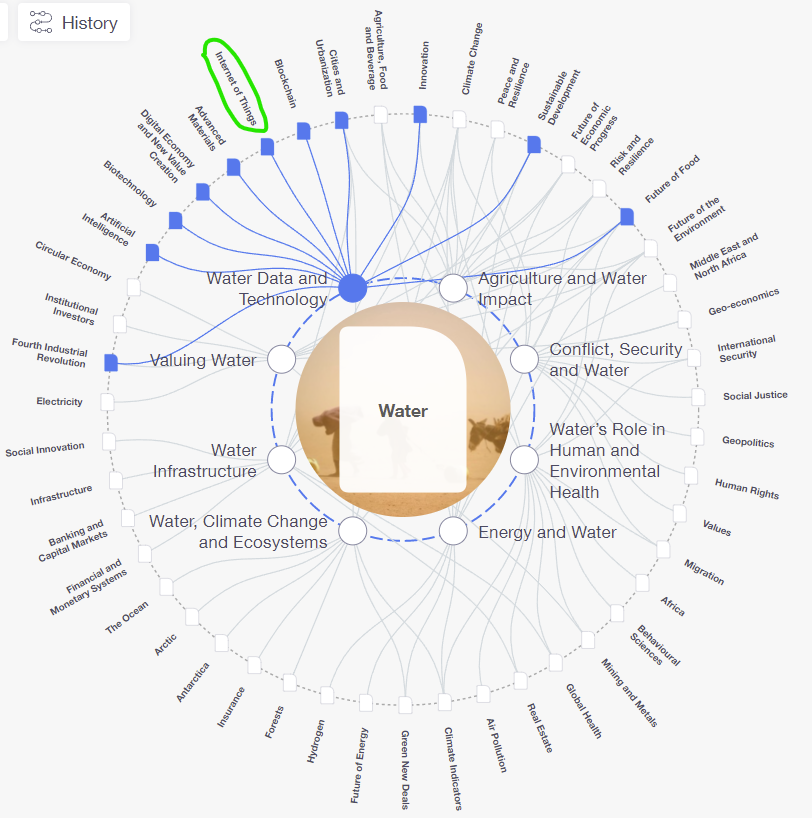
\includegraphics[width=1\textwidth]{./Figuras/WEFoum-Water-IoT.png} 
\caption{Diagrama del \textit{World Economic Forum} sobre los aspectos del agua en el mundo de hoy. Se hace énfasis en su relación de las tecnologías emergentes.}
\label{fig:WEFoum-Water-IoT}
\end{figure}

\pagebreak 

En las ciudades, con la complejidad de las redes urbanas de agua potable y la multiplicación de puntos de agua, también se incrementan las fugas por agrietamiento o rotura de las tuberías. Se estima que estos eventos representan un 20\% del agua perdida. Ante eventos de esta naturaleza, dependiendo de la magnitud de la fuga, si se tratara por ejemplo, de la rotura de la tubería alimentadora de una casa, la inundación será advertida rápidamente por sus residentes. Sin embargo, si las fugas fueran ligeras, será difícil tener una detección temprana. Por lo tanto, las acciones correctivas tomarán tiempo en ejecutarse.

Para un mejor entendimiento, se puede hacer un cálculo sencillo para identificar la cantidad de agua que se podría desperdiciar en un hogar que tuviera un solo punto de agua defectuoso, y que pierda 30 gotas por minuto. Este ritmo podría pasar inadvertido por el propietario, pero sí logrará perder alrededor de 43200 gotas al día, lo que equivale a 10 litros. Anualizado este cálculo, se llega a 3650 litros al año de agua perdida.

La necesidad principal a satisfacer en el mercado es la carencia de información en tiempo real que permita la rápida atención de fugas y prevenga el desperdicio de agua potable en los hogares u organizaciones.


\textbf{Solución planteada en proyecto a realizar} 

El proyecto busca construir un prototipo de sistema que permita el control del consumo de agua potable y la detección de fugas en redes caseras o residenciales. 

El proyecto propuesto se abordará con un sensor inalámbrico de caudal de agua que permita la lectura del caudal que pasa por el punto monitoreado. Los datos deberán ser enviados a través del protocolo MQTT para su almacenamiento en una base de datos. En el frente de visualización de la información, se propone la creación de una aplicación que permita mostrar el flujo de agua en el punto monitoreado, así como su consumo acumulado durante un período de tiempo definido. 

El principal desafío del presente proyecto es la identificación del sensor que permita la correcta medición del flujo de agua. En el mercado existe disponibilidad de contadores de caudal de agua. Sin embargo, se trata de sensores intrusivos, ya que requieren alterar la plomería para incorporarlos. Se busca que el proyecto no sea intrusivo para una fácil utilización. Para lograr este objetivo, se necesitará usar dispositivos que utilicen la técnica de ultrasonido, que si bien existen en el mercado, no lo hace de forma masiva.

Los contadores inteligentes de caudal de agua poseen tecnología madura que las empresas que gestionan el agua potable en las ciudades, como AySA, irán desplegando paulatinamente. A mediano/largo plazo, estos dispositivos enviarán la información en tiempo real a sus sistemas centrales y eventualmente, se compartirá con los usuarios finales.

La motivación del presente proyecto es poder brindar al mercado una herramienta económica para la medición de caudal en tiempo real. Esta solución podrá estar disponible para hogares, organizaciones o para quienes brinden servicios relacionados. Se podrá conocer de forma temprana el consumo actual y detectar, basándose en comparación de consumos anteriores, fugas de agua potable.

En la figura \ref{fig:diagHLSolucion} se presenta el diagrama a alto nivel de la solución.


%\vspace{25px}

\begin{figure}[htpb]
\centering 
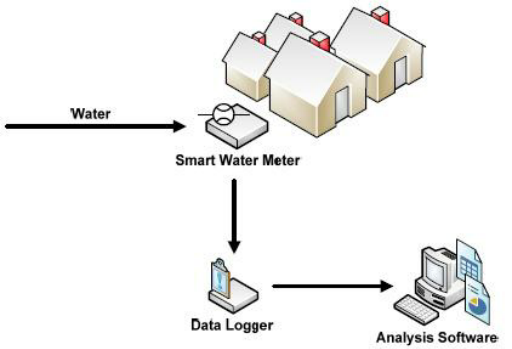
\includegraphics[width=.8\textwidth]{./Figuras/diagHLSolucion.png} 
\caption{Diagrama a alto nivel de la solución.}
\label{fig:diagHLSolucion}
\end{figure}

\vspace{25px}

\end{consigna}


\section{2. Identificación y análisis de los interesados}
\label{sec:interesados}

\begin{consigna}{black} 

\begin{table}[ht]
%\caption{Identificación de los interesados}
%\label{tab:interesados}
\begin{tabularx}{\linewidth}{@{}|l|X|X|l|@{}}
\hline
\rowcolor[HTML]{C0C0C0} 

Rol           & Nombre y Apellido & Organización 	& Puesto 	\\ \hline
Cliente       & Marleny López Machuca & Cliente particular	& -- 	\\ \hline
Responsable   & \authorname       & FIUBA 			& Alumno 	\\ \hline
Orientador    & \supname       & \pertesupname  	& Director  \\ \hline %\pertesupname
Colaborador   & \cosupname       & \pertecosupname     & Co-director \\ \hline

\end{tabularx}
\end{table}

 
\begin{itemize}
	\item Orientador: posee conocimiento y experiencia en soluciones TI que ayudará en la estrategia y definición de los objetivos del proyecto. Cuenta con escaso tiempo disponible. Se deberán planificar reuniones con anticipación de 15 días.
	\item Colaborador: posee conocimiento y experiencia en soluciones IoT que ayudará en los conceptos y aspectos técnicos del proyecto. Cuenta con escaso tiempo disponible. Se deberán planificar reuniones con anticipación de 15 días.
\end{itemize}

\end{consigna}



\section{3. Propósito del proyecto}
\label{sec:proposito} 
\begin{consigna}{black}
El propósito del proyecto es la construcción de un prototipo de sistema que permita el control del consumo de agua potable y la detección de fugas en redes caseras o empresariales. 

A través de una solución profesional, simple y práctica, se busca minimizar la falta de información en tiempo real de la pérdida de agua que existe en los hogares y eventualmente a industrias y otros sectores. Esto podrá contribuir, en algo, a la sensibilización de estas pérdidas del líquido vital.

A nivel académico, el propósito es mejorar el conocimiento sobre sensorización de caudal de fluidos, específicamente de agua. Se busca ampliar el conocimiento en la integración de los componentes de medición, protocolos de comunicación y servicios de software que pongan en valor la información sobre el consumo de agua potable.
\end{consigna}

\section{4. Alcance del proyecto}
\label{sec:alcance}

\begin{consigna}{black}

El presente proyecto tiene como alcance:

\begin{enumerate}
\item Diseño, identificación e implementación de prototipo de solución de telemetría para medición de caudal de agua en una tubería residencial de hasta 1'' de diámetro:
\begin{itemize}
	\item Que esté basada en utilización de sensores de medición de caudal de agua con tecnología ultrasónica.
	\item Donde los sensores no sean instalados \textquotedblleft{en línea}\textquotedblright  en la tubería o cañería, sino que sean instalados de forma no intrusiva, es decir, sin intervenirla.
	\item En la que la comunicación hacia la solución de software sea inalámbrica, utilizando preferentemente protocolo Wi-Fi.
\end{itemize}

\item Diseño y construcción de un prototipo de software para la captura y procesamiento de datos que estará basado en tecnología de contenedores.

\item Diseño y construcción de un prototipo de software front-end para la presentación de datos en tiempo real y de forma histórica.

\end{enumerate}

El presente proyecto no incluye:

\begin{itemize}
	\item Detección de caudal de otro tipo de fluidos.
	\item Inclusión de servicios de nube.
	\item Gestión de analítica de datos.
\end{itemize}

\textbf{Beneficios.}  
Los beneficios de este producto son:
\begin{itemize}
	\item Instrumento no intrusivo a la cañería.
	\item Dispositivo ligero y manejable.
	\item Rápida programación e instalación.
	\item Amplia aplicación en cañerías hasta de 1'' ubicables en distintos sectores.
	\item Detección de flujo de agua en tiempo real.
\end{itemize}
\end{consigna}


\section{5. Supuestos del proyecto}
\label{sec:supuestos}

\begin{consigna}{black}
Para el desarrollo del presente proyecto se supone que: 

\begin{itemize}
	\item Se dispondrá de tiempo suficiente para el cumplimiento de los objetivos y entregables.
	\item Se dispondrá de los recursos económicos suficientes para la adquición de los materiales necesarios para la construcción del prototipo y software asociado.
	\item Se dispondrá de los recursos técnicos suficientes y oportunamente para la construcción del prototipo en tiempo y forma.
	\item Se dispondrá de orientación oportuna por parte de todos los involucrados de acuerdo a su rol.
	\item Los niveles de precisión de los dispositivos de telemetría elegidos están dentro del rango del 95\%.
	\item Se dispondrá de red inalábrica Wi-Fi con nivel de recepción de señal aceptable (-60 dBm).
\end{itemize}

\end{consigna}

\section{6. Requerimientos}
\label{sec:requerimientos}

\begin{consigna}{black}
Los requerimientos del proyecto serán listados de acuerdo al siguiente criterio:
\begin{itemize}
	\item Su clasificación será: funcionales, interfases, testing y documentación.
	\item La prioridad de los requerimientos se listan de mayor a menor.
	\item El cumplimiento de estos requerimientos es mandatorio, salvo se especifique si fuera opcional.
\end{itemize}

\begin{enumerate}

\item Requerimientos funcionales:
	\begin{enumerate}
		\item La conexión de los dispositivos debe ser de forma inalámbrica.
		\item Los dispositivos de medición de caudal de agua deberán usar tecnología ultrasónica.
		\item El sistema debe atender las salidas de agua de servicios higiénicos y/o de tuberías de hasta 1".
		\item La transmisión de datos debe ser ligera y debe consumir baja energía. 
		\item El software embebido debe poder encapsularse en un contenedor docker.
		\item El sistema debe incluir notificaciones que permitan alertar a usuarios de la alteración del caudal cuando supere el 10\% al promedio histórico.	
		\item Los sensores deberán conectarse a una red de forma predeterminada.	
		\item Opcionalmente, el sistema debe tener capacidad portátil para conexión de datos, alimentación eléctrica e instalación de plomería.
		\item Opcionalmente, el sistema debe adecuarse a los lineamientos establecidos en la ISO 30141:2018.
	\end{enumerate}

\item Requerimientos de interfases:
	\begin{enumerate}
		\item La aplicación debe funcionar en los navegadores web Chrome y Mozilla.
		\item La aplicación web debe funcionar de forma responsiva en dispositivos Android e iOS.
		\item La aplicación web debe permitir el registro de ubicación del sensor y asociarla con la colección de datos.
		\item La aplicación web debe mostrar el caudal de agua de cada sensor en tiempo real. 
		\item La aplicación web debe mostrar el caudal histórico de cada sensor y el promedio de los últimos 7 días.
		\item Opcionalmente, el sistema tendrá control de accesos configurable.
	\end{enumerate}

\item Requerimientos de testing:
	\begin{enumerate}
		\item El aplicativo web tendrá un banco de pruebas unitarias para aseguramiento de calidad y funcionamiento.
		\item El dispositivo de telemetría tendrá un banco de pruebas unitarias para aseguramiento de calidad y funcionamiento.
		\item El sistema en general tendrá un banco de pruebas integrables.
	\end{enumerate}

\item Requerimientos de documentación:
	\begin{enumerate}
		\item Documentación con arquitectura técnológica y funcional.
		\item El sistema debe contar con documentación de cobertura de señal. 
		\item El sistema debe incluir documentación con estudio de parámetro para medición de caudal de agua usando sensores ultrasónicos.
		\item Desarrollo web deberá estar documentado bajo el método de anotaciones.
		\item Documentación de plan de pruebas y resultados.
		\item Video demostrativo de uso del prototipo.
		\item Informe final.
		\item Se utilizará un sistema de control de versiones.
	\end{enumerate}

\end{enumerate}

\end{consigna}

\section{7. Historias de usuarios (\textit{Product backlog})}
\label{sec:backlog}

\begin{consigna}{black}
A continuación se listan las historias de usuario y su ponderación, que es un número entero que representa el tamaño de la historia comparada con otras historias de similar tipo. Está basada en la serie de Fibonacci.

Los criterios para la ponderación son los siguientes:

\begin{table}[ht]
\label{tab:haUsuarioPesos}
\centering
\begin{tabularx}{\linewidth}{@{}|c|X|c|@{}}
\hline
\rowcolor[HTML]{C0C0C0} 
\# & \multicolumn{1}{c|}{\cellcolor[HTML]{C0C0C0}Criterio} 	& Peso      \\ \hline
1      & \textbf{Dificultad del trabajo a realizar}          	&  \\ \hline 
      	& Bajo                 								&  1 \\ \hline
       	& Medio                								&  3 \\ \hline
      	& Alto                 								&  5 \\ \hline
2      & \textbf{Complejidad del trabajo a realizar}        	&  \\ \hline 
      	& Bajo                 								&  1 \\ \hline
       	& Medio                								&  5 \\ \hline
      	& Alto                 								& 13 \\ \hline
2      & \textbf{Riesgo-incertidumbre del trabajo a realizar}        	&  \\ \hline 
      	& Bajo                 								&  1 \\ \hline
       	& Medio                								&  5 \\ \hline
      	& Alto                 								& 13 \\ \hline

\end{tabularx}
\end{table}

\pagebreak 
Las historias de usuario son las siguientes:

\begin{enumerate}
\item Como usuario final quiero que la medición del caudal sea lo más precisa posible para tener confianza en la solución y compararla con mediciones de la empresa de suministro de agua.
	\begin{itemize}
		\item Dificultad	:  5
		\item Complejidad	:  8
		\item Riesgo		: 13
		\item Total			: 26
		\item \textbf{\textit{Story Points	:} 34} 		
	\end{itemize}

\item Como usuario final quiero que la aplicación web sea responsiva para que sea usada desde computadoras y móviles.
	\begin{itemize}
		\item Dificultad	:  3
		\item Complejidad	:  8
		\item Riesgo		:  5
		\item Total			: 16
		\item \textbf{\textit{Story Points	:} 21}		
	\end{itemize}

\item Como usuario final deseo que la solución proporcione información histórica por ubicación del sensor para poder comparar con consumos pasados.
	\begin{itemize}
		\item Dificultad	:  4
		\item Complejidad	: 10
		\item Riesgo		:  7
		\item Total			: 21
		\item \textbf{\textit{Story Points	:} 21}		
	\end{itemize}

\item Como usuario final deseo que la solución notifique ante alteración del patrón de consumo cuando se desvíe en al menos un 10\% respecto al consumo histórico para tener una alerta temprana de posibles fugas.
	\begin{itemize}
		\item Dificultad	:  5
		\item Complejidad	: 15
		\item Riesgo		: 10
		\item Total			: 30
		\item \textbf{\textit{Story Points	:} 34}		
	\end{itemize}
	
\item Como usuario final deseo que la solución sea portátil para poder moverla a distintos ambientes.
	\begin{itemize}
		\item Dificultad	:  4
		\item Complejidad	:  5
		\item Riesgo		: 13
		\item Total			: 24
		\item \textbf{\textit{Story Points	:} 34}		
	\end{itemize}
\end{enumerate}

\end{consigna}

\section{8. Entregables principales del proyecto}
\label{sec:entregables}

\begin{consigna}{black}

Los entregables del proyecto son:

\begin{itemize}
	\item Prototipo final de solución.
	\item Aplicación web implementada.
	\item Documentación del proyecto:
	\begin{itemize}
		\item Diagrama de arquitectura de solución.
		\item Diagrama de circuitos esquemáticos.
		\item Código fuente del software.
		\item Diagrama de instalación.
		\item Memoria técnica final.
	\end{itemize}
	
\end{itemize}

\end{consigna}

\section{9. Desglose del trabajo en tareas}
\label{sec:wbs}

\begin{consigna}{black}

\begin{enumerate}
\item \textbf{Planificación del proyecto: 40 hs}
	\begin{enumerate}
	\item Elaboración del plan de proyecto (20 hs).
	\item Análisis de factibilidad (10 hs).
	\item Validaciones de calidad (10 hs).
	\end{enumerate}
\item \textbf{Investigación inicial: 60 hs}
	\begin{enumerate}
	\item Investigación sobre sensores de medición de flujo de agua con tecnología ultrasónica (30 hs).
	\item Indagación sobre nivel de programación de sensores identificados (20 hs).
	\item Proceso de adquisición de sensores (10 hs).
	\end{enumerate}
\item \textbf{Diseño de arquitectura de solución: 60 hs}
	\begin{enumerate}
	\item Arquitectura tecnológica (15 hs).
	\item Arquitectura de aplicación (20 hs).
	\item Arquitectura de integración (10 hs).
	\item Arquitectura de datos (15 hs).
	\end{enumerate}
\item \textbf{Desarrollo de aplicación web: 150 hs}
	\begin{enumerate}
	\item Desarrollo front end (50 hs).
	\item Desarrollo back end (60 hs).
	\item Pruebas unitarias de aplicación (30 hs).
	\item Habilitación de infraestructura (10 hs).
	\end{enumerate}
\item \textbf{Desarrollo de sistema embebido: 150 hs}
	\begin{enumerate}
	\item Desarrollo de algoritmo de medición de caudal de agua (50 hs).
	\item Desarrollo de algoritmo de comunicaciones (40 hs).
	\item Encapsulamiento de aplicación en contenedores (20 hs).
	\item Pruebas unitarias de sistema embebido en dispositivo de telemetría (40 hs).
	\end{enumerate}
\item \textbf{Integración y pruebas integrales: 100 hs}
	\begin{enumerate}
	\item Integración de componentes (40 hs).
	\item Pruebas integrales de sistema y corrección de errores (60 hs).
	\end{enumerate}
\item \textbf{Elaboración de documentación: 100 hs}
	\begin{enumerate}
	\item Confección de memoria técnica (60 hs).
	\item Informes de avance (20 hs).
	\item Presentación de defensa (20 hs).
	\end{enumerate}
\end{enumerate}

\textbf{Cantidad total de horas: 660 hs}

\end{consigna}

\section{10. Diagrama de Activity On Node}
\label{sec:AoN}

\begin{consigna}{black}
El proyecto tiene dos líneas de actividades paralelas, que son:
\begin{itemize}
		\item Actividades de planeamiento, diseño, desarrollo de aplicación web y back-end. 
		\item Actividades asociadas a la investigación, adquisición de sensores y desarrollo del sistema embebido.
\end{itemize}

La ruta crítica incluye la primera línea de actividades, aquellas de mayor complejidad y dificultad, hasta el final del proyecto.

Se presenta el diagrama de \textit{Activity On Node} a partir del WBS definido en la etapa anterior. Las unidades mostradas en la gráfica están expresadas en \textbf{horas} y la ruta crítica se muestra con las flechas azules.


%La figura \ref{fig:AoN} fue elaborada con el paquete latex tikz y pueden consultar la siguiente referencia \textit{online}:

%\url{https://www.overleaf.com/learn/latex/LaTeX_Graphics_using_TikZ:_A_Tutorial_for_Beginners_(Part_3)\%E2\%80\%94Creating_Flowcharts}

\end{consigna}

%\begin{figure}[htpb]
%\centering 
%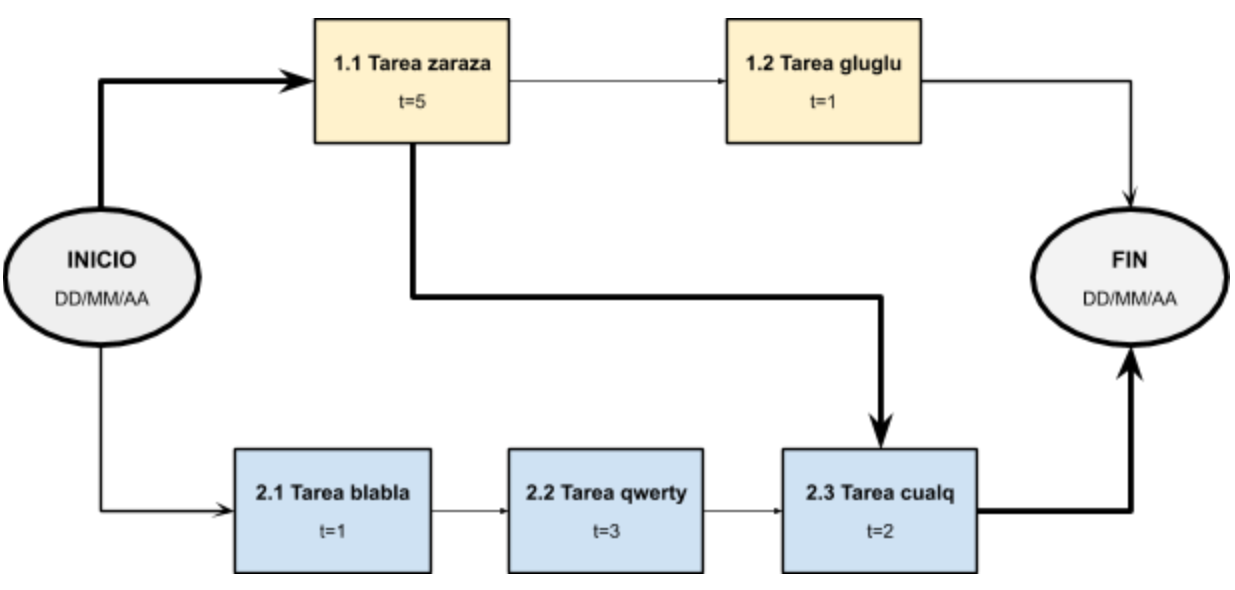
\includegraphics[width=.8\textwidth]{./Figuras/AoN.png}
%\caption{Diagrama en \textit{Activity on Node}}
%\label{fig:AoN}
%\end{figure}

\begin{landscape}

\begin{figure}[htpb]
\centering 
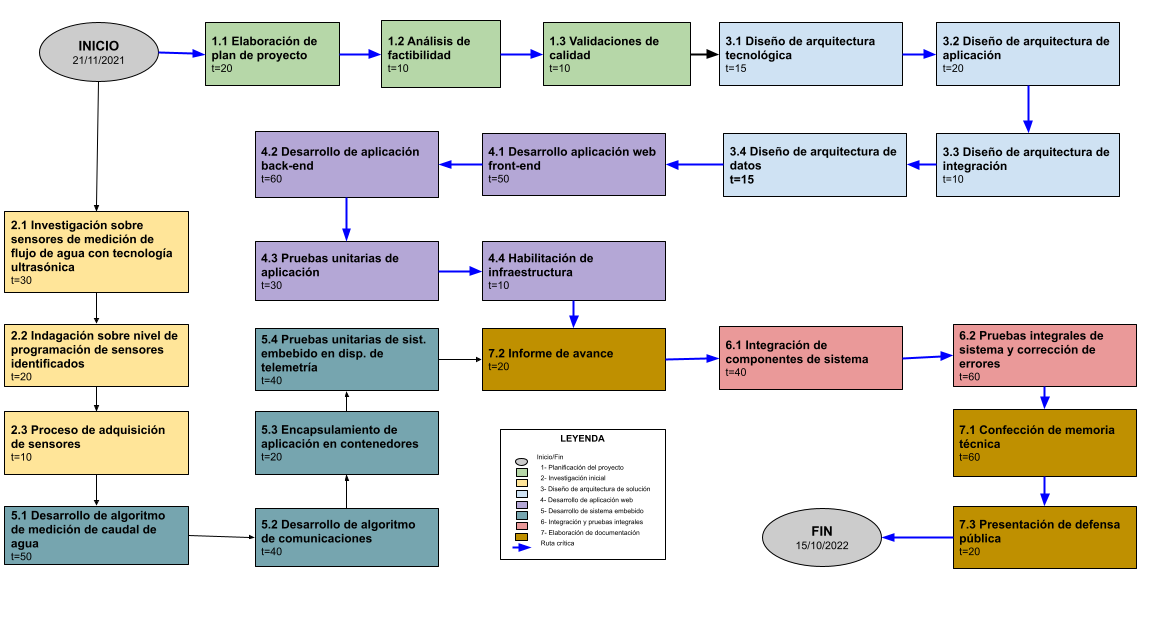
\includegraphics[scale=.6]{./Figuras/TF_MonAgua_AoN.png} 
\caption{Diagrama en \textit{Activity on Node}.}
\label{fig:AoN}
\end{figure}
\end{landscape}


\section{11. Diagrama de Gantt}
\label{sec:gantt}

\begin{consigna}{black}

A continuación en la figura \ref{fig:ListaGantt} se listan las actividades con las fechas de inicio y fin establecidas para el proyecto. Se tienen en cuenta las siguientes consideraciones:

\begin{itemize}
		\item La asignación de un (01) recurso de tipo desarrollador.
		\item El trabajo diario será de tres (03) horas por seis (06) días por semana.
		\item Vacaciones desde el 15 de diciembre de 2021 al 28 de febrero de 2022 y desde el 11 al 22 de julio de 2022.
\end{itemize}

\begin{figure}[htpb]
\centering 
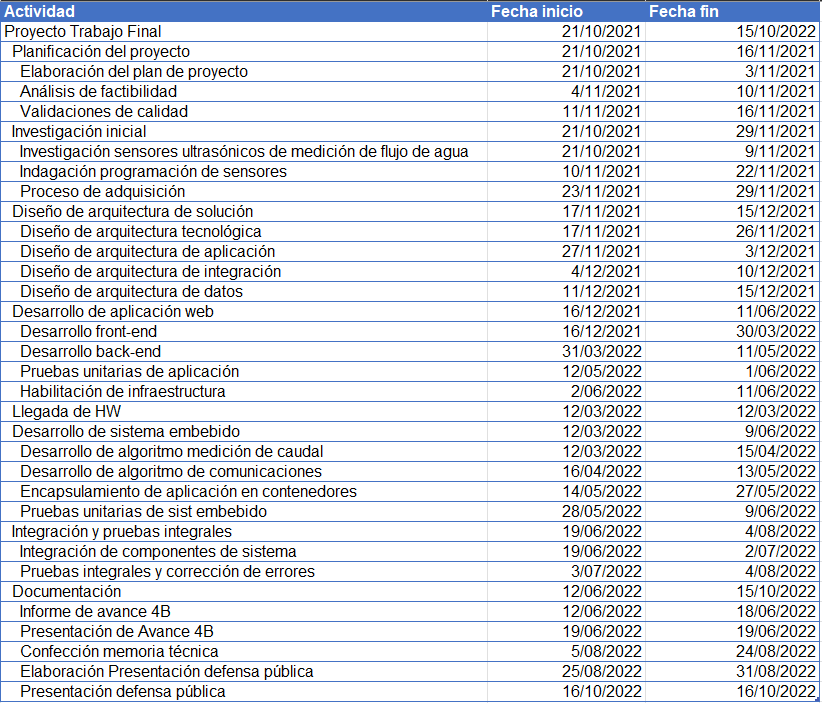
\includegraphics[scale=.7]{./Figuras/TF-gantt-lista.png} 
\caption{Diagrama de listado de actividades.}
\label{fig:ListaGantt}
\end{figure}


En las figuras \ref{fig:diagGantt1} y \ref{fig:diagGantt2} se muestra el diagrama de Gantt realizado para el proyecto.
%con el paquete de \textit{pgfgantt}. En la plantilla pueden ver el código que lo genera y usarlo de base para construir el propio.

%\begin{figure}[htbp]
%\begin{center}
%\begin{ganttchart}{1}{12}
%  \gantttitle{2020}{12} \\
%  \gantttitlelist{1,...,12}{1} \\
%  \ganttgroup{Group 1}{1}{7} \\
%  \ganttbar{Task 1}{1}{2} \\
%  \ganttlinkedbar{Task 2}{3}{7} \ganttnewline
%  \ganttmilestone{Milestone o hito}{7} \ganttnewline
%  \ganttbar{Final Task}{8}{12}
%  \ganttlink{elem2}{elem3}
%  \ganttlink{elem3}{elem4}
%\end{ganttchart}
%\end{center}
%\caption{Diagrama de gantt de ejemplo}
%\label{fig:gantt}
%\end{figure}


%\begin{landscape}
\begin{figure}[htpb]
\centering 
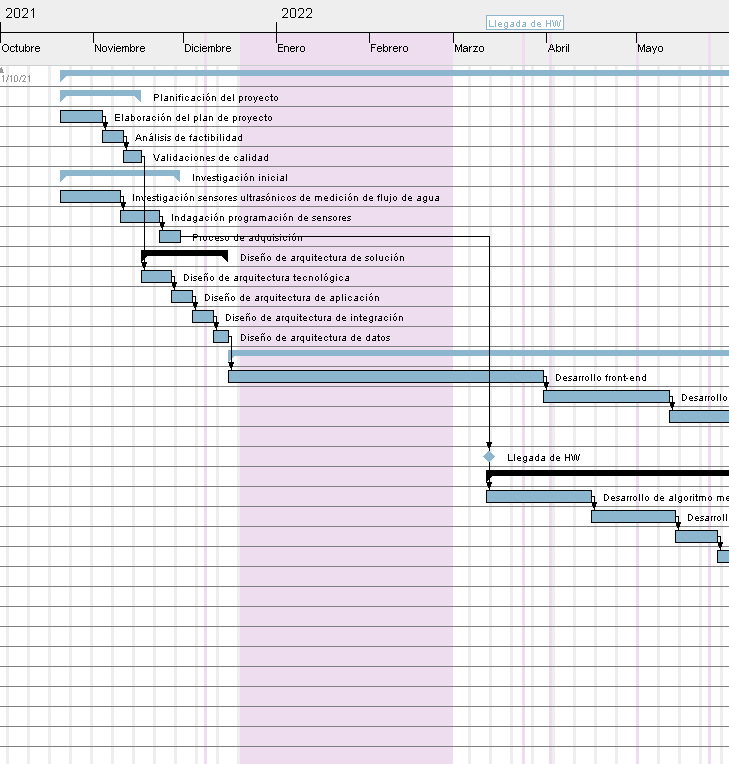
\includegraphics[height=.7\textheight]{./Figuras/TF-gantt1.png}
\caption{Diagrama de Gantt: octubre 2021 - mayo 2022.}
\label{fig:diagGantt1}
\end{figure}

\begin{figure}[htpb]
\centering 
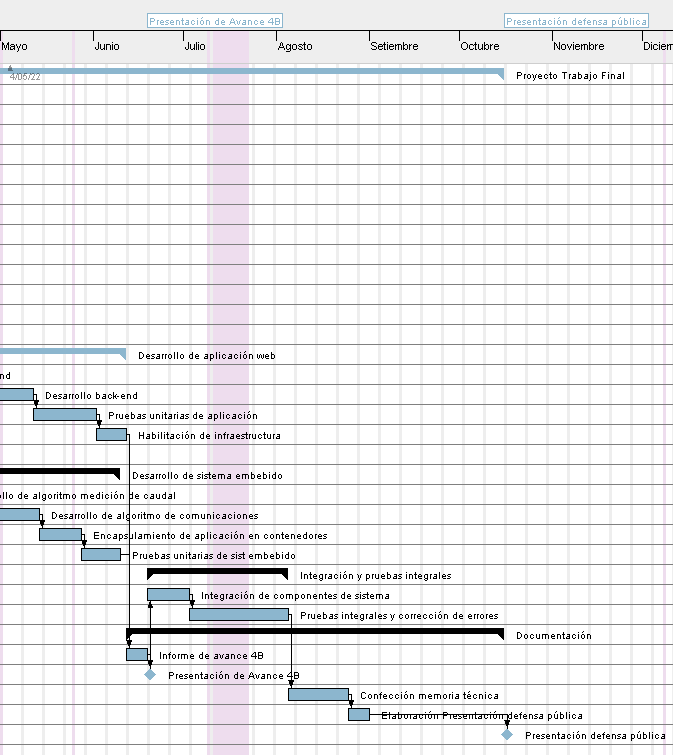
\includegraphics[height=.7\textheight]{./Figuras/TF-gantt2.png}
\caption{Diagrama de Gantt: mayo - diciembre 2022.}
\label{fig:diagGantt2}
\end{figure}

%\end{landscape}

\end{consigna}


\section{12. Presupuesto detallado del proyecto}
\label{sec:presupuesto}

\begin{consigna}{black}
Se presenta el presupuesto del proyecto. Está expresado en dólares americanos (USD). Cotización del 21/11: \$100.58.

\end{consigna}

\begin{table}[htpb]
\centering
\begin{tabularx}{\linewidth}{@{}|X|c|r|r|@{}}
\hline
\rowcolor[HTML]{C0C0C0} 
\multicolumn{4}{|c|}{\cellcolor[HTML]{C0C0C0}COSTOS DIRECTOS} \\ \hline
\rowcolor[HTML]{C0C0C0} 
Descripción &
  \multicolumn{1}{c|}{\cellcolor[HTML]{C0C0C0}Cantidad} &
  \multicolumn{1}{c|}{\cellcolor[HTML]{C0C0C0}Valor unitario} &
  \multicolumn{1}{c|}{\cellcolor[HTML]{C0C0C0}Valor total} \\ \hline
\multicolumn{1}{|l|}{Servicios de ingeniería} & 660 hs
   & 10.00
   & 6600.00
   \\ \hline
\multicolumn{1}{|l|}{Sensor de caudal de agua ultrasónico} & 01 un
   & 110.00
   & 110.00
   \\ \hline
\multicolumn{1}{|l|}{Unidad de cómputo Raspberry Pi} & 01 un
   & 130.00
   & 130.00
   \\ \hline


\multicolumn{3}{|c|}{SUBTOTAL} &
  \multicolumn{1}{r|}{6840.00} \\ \hline
\rowcolor[HTML]{C0C0C0} 
\multicolumn{4}{|c|}{\cellcolor[HTML]{C0C0C0}COSTOS INDIRECTOS} \\ \hline
\rowcolor[HTML]{C0C0C0} 
Descripción &
  \multicolumn{1}{c|}{\cellcolor[HTML]{C0C0C0}Cantidad} &
  \multicolumn{1}{c|}{\cellcolor[HTML]{C0C0C0}Valor unitario} &
  \multicolumn{1}{c|}{\cellcolor[HTML]{C0C0C0}Valor total} \\ \hline
\multicolumn{1}{|l|}{20\% de costo directo} & 01
   & 1368.00
   & 1368.00
   \\ \hline

\multicolumn{3}{|c|}{SUBTOTAL} &
  \multicolumn{1}{r|}{1368.00} \\ \hline
\rowcolor[HTML]{C0C0C0}
\multicolumn{3}{|r|}{TOTAL} & 8208.00
   \\ \hline
\end{tabularx}%
\end{table}


\section{13. Gestión de riesgos}
\label{sec:riesgos}

\begin{consigna}{black}
En esta sección se identificarán y evaluarán los riesgos del proyecto. La escala de medición será del 1 al 10:
\begin{itemize}
	\item Severidad (S): mientras más severo, más alto es el número.\\
	\item Probabilidad de ocurrencia (O): mientras más probable, más alto es el número.\\
\end{itemize}   


a) Identificación de los riesgos y estimación de sus consecuencias:
 
Riesgo 1: no contar oportunamente con componentes de hardware necesarios.
\begin{itemize}
	\item Severidad (S): 10. \\
	Retraso de llegada de componentes alterará cronograma establecido.
	\item Probabilidad de ocurrencia (O): 7. \\
	Es variable, debido a la situación actual en el mundo pueden ocurrir retrasos en la entrega de componentes, y por lo tanto la probabilidad de ocurrencia es elevada.
\end{itemize}   

Riesgo 2: errónea elección de sensores ultrasónicos.
\begin{itemize}
	\item Severidad (S): 10. \\
	Implica un trabajo de menor calidad o tener que realizar una nueva búsqueda de sensores y por consiguiente una demora en el cronograma establecido.
	\item Ocurrencia (O): 4. \\
	Es baja, ya que se verificarán las especificaciones técnicas disponibles para la correcta elección.
\end{itemize}

Riesgo 3: imposibilidad o alta complejidad de programación de los sensores ultrasónicos.
\begin{itemize}
	\item Severidad (S): 10. \\
	La alta complejidad de programación acarreará la nueva elección de componentes y el consecuente retraso en el cronograma establecido.
	\item Ocurrencia (O): 6. \\
	La documentación disponible de los dispositivos adquiridos podría no contemplar métodos de programación soportados por estos.
\end{itemize}

Riesgo 4: bajo nivel de soporte para desarrollo de algoritmos de detección de flujo de agua.
\begin{itemize}
	\item Severidad (S): 5. \\
	Implica la búsqueda de nuevas alternativas para replantear algoritmos y/o la elección de nuevo dispositivo más fiable.
	\item Ocurrencia (O): 4. \\
	Para la elección de los dispositivos se tomará en cuenta el nivel de precisión de acuerdo a los requerimientos fijados. En las pruebas unitarias deberá evaluarse si los algoritmos aplicados permiten una correcta precisión.
\end{itemize}

Riesgo 5: fallo de dispositivos de hardware por mala manipulación.
\begin{itemize}
	\item Severidad (S): 10. \\
	La incorrecta manipulación del dispositivo que ocasione su falla impactará actividades por nueva adquisición de este y retrasará el cronograma establecido.
	\item Ocurrencia (O): 4. \\
	Solo una persona tendrá acceso a los dispositivos y se tomarán medidas para evitar fallo por descargas electroestáticas.
\end{itemize}

Riesgo 6: estimación incorrecta de tiempo de desarrollo de aplicaciones.
\begin{itemize}
	\item Severidad (S): 9. \\
	Implica la no entrega del proyecto a tiempo.
	\item Ocurrencia (O): 10. \\
	Inexperiencia en desarrollo de aplicaciones y el poco tiempo disponible incrementan la probabilidad de ocurrencia.
\end{itemize}



b) Tabla de gestión de riesgos:      

En la gestión de riesgos, se calculará el RPN (número de prioridad de riesgo) a partir de la multiplicación de los números dados en la severidad y la ocurrencia. El RPN se formula como RPN=SxO.

\begin{table}[htpb]
\centering
\begin{tabularx}{\linewidth}{@{}|X|c|c|c|c|c|c|@{}}
\hline
\rowcolor[HTML]{C0C0C0} 
Riesgo & S & O & RPN &	 S* & O* & RPN* \\ \hline
1: No contar oportunamente con componentes de hardware necesarios   & 10  &  7 & \cellcolor{red}{70}  &  3  & 6   & 18     \\ \hline
2: Errónea elección de sensores ultrasónicos       & 10  &  4 & 40    &  -  &  -  &  -    \\ \hline
3: Imposibilidad o alta complejidad de programación de los sensores ultrasónicos       & 10  &  6 & \cellcolor{red}{60}  & 10   & 4   & 40     \\ \hline
4: Bajo nivel de soporte para desarrollo de algoritmos de detección de flujo de agua       &  5 & 4  & 20  & -   & -   & -     \\ \hline
5: Fallo de dispositivos de hardware por mala manipulación       & 10  & 4  & 40    & -   & -   & -     \\ \hline
6: Estimación incorrecta de tiempo de desarrollo de aplicaciones       &  9   & 10  & \cellcolor{red}{90}    & 5   & 8   & 40     \\ \hline
\end{tabularx}%
\end{table}

Criterio adoptado: 
Se tomarán medidas de mitigación en los riesgos cuyos números de RPN sean mayores a 50.

Nota: los valores marcados con (*) en la tabla corresponden luego de haber aplicado la mitigación.

c) Plan de mitigación de los riesgos que originalmente excedían el RPN máximo establecido:
 
Se mostrarán los planes de mitigación de los riesgos 1, 3 y 6. 
 
Riesgo 1: evaluar y adquirir lo antes posible los dispositivos necesarios para tenerlos oportunamente considerando el tiempo de transporte. \\
  - Severidad (S): 3. \\
	Retraso de llegada de componentes alterará cronograma establecido. \\
  - Probabilidad de ocurrencia (O): 6. \\
	Riesgo es mitigado con tiempo de anticipación de la compra. \\

Riesgo 3: revisión de reseñas y alternativa de implementar el sistema en un dispositivo de la familia Raspberry. \\
  - Severidad (S): 10. \\
	Se mantiene igual. La alta complejidad de programación acarreará la nueva elección de componentes y retraso en el cronograma establecido. \\
  - Probabilidad de ocurrencia (O): 4. \\
	Evaluación de capacidad de programación en dispositivo deberá reducir riesgo. \\

Riesgo 6: solicitud de apoyo con recurso alterno para cerrar brechas de programación. \\ 
  - Severidad (S): 9. \\
	Se mantiene igual. Implica la no entrega del proyecto a tiempo. \\
  - Probabilidad de ocurrencia (O): 4. \\
	Contar con respaldo para avance de actividad reduce la probabilidad de ocurrencia. \\

\end{consigna}


\section{14. Gestión de la calidad}
\label{sec:calidad}

\begin{consigna}{black}
Para cada uno de los requerimientos del proyecto se indican la verificación y validación correspondientes:

\begin{enumerate}
\item Requerimientos funcionales:
	\begin{enumerate}
		\item La conexión de los dispositivos debe ser de forma inalámbrica.
			\begin{itemize}
				\item Verificación técnica de conectividad con dirección MAC registrada en AP usando protocolo WiFi. 
				\item Validación con el cliente con conexión de dispositivo a red inalámbrica.
			\end{itemize}
		\item Los dispositivos de medición de caudal de agua deberán usar tecnología ultrasónica.
			\begin{itemize}
				\item Verificación de especificaciones técnicas de dispositivo. 
				\item Validación de referencia de caja o afiche comercial de dispositivo con mención a dicha tecnología.  
			\end{itemize}
		\item El sistema debe atender las salidas de agua de servicios higiénicos y/o de tuberías de hasta 1".
			\begin{itemize}
				\item Verificación de especificaciones técnicas de dispositivo.  
				\item Validación con el cliente para confirmar que dispositivo soporta conectarse a tuberías hasta de dicho diámetro.
			\end{itemize}
		\item La transmisión de datos debe ser ligera y debe consumir baja energía. 
			\begin{itemize}
				\item Verificación de especificaciones técnicas de dispositivo y/o medición de tráfico usando algún capturador de paquetes. 
				\item Validación con el cliente de confirmación con especialista. 
			\end{itemize}
		\item El software embebido debe poder encapsularse en un contenedor docker.
			\begin{itemize}
				\item Verificación técnica de archivo de configuración docker. 
				\item Validación con el cliente de poder ejecutar la lógica en un solo contenedor.
			\end{itemize}
		\item El sistema debe incluir notificaciones que permitan alertar a usuarios de la alteración del caudal cuando supere el 10\% al promedio histórico.	
			\begin{itemize}
				\item Verificación en simulación de evento de superación de umbral. 
				\item Validación con el cliente de llegada de notificación. 
			\end{itemize}
		\item Los sensores deberán conectarse a una red de forma predeterminada.	
			\begin{itemize}
				\item Verificación técnica que sensor tiene configuración predeterminada activa en settings del dispositivo. 
				\item Validación con el cliente de que dispositivo no pregunta a qué red conectarse. 
			\end{itemize}
		\item Opcionalmente, el sistema debe tener capacidad portátil para conexión de datos, alimentación eléctrica e instalación de plomería.
			\begin{itemize}
				\item Verificación de especificaciones técnicas de todas o algunas de los requerimientos opcionales. 
				\item Validación de portabilidad de dispositivo.  
			\end{itemize}
		\item Opcionalmente, el sistema debe adecuarse a los lineamientos establecidos en la ISO 30141:2018.
			\begin{itemize}
				\item Verificación de documentación del proyecto que haga referencia a la ISO. 
				\item Validación en documentación de ISO de las referencias mencionadas.
			\end{itemize}
	\end{enumerate}

\item Requerimientos de interfases:
	\begin{enumerate}
		\item La aplicación debe funcionar en los navegadores web Chrome y Mozilla.
			\begin{itemize}
				\item Verificación de la ejecución de la aplicación en una computadora usada en el proyecto con ambos navegadores.
				\item Validación con el cliente para confirmar compatibilidad en una computadora de terceros. 
			\end{itemize}
		\item La aplicación web debe funcionar de forma responsiva en dispositivos Android e iOS.
			\begin{itemize}
				\item Verificación de la ejecución de la aplicación en simuladores de Android y iOS.
				\item Validación con el cliente para confirmar compatibilidad en el celular del cliente. 
			\end{itemize}
		\item La aplicación web debe permitir el registro de ubicación del sensor y asociarla con la colección de datos.
			\begin{itemize}
				\item Verificación de query con id de sensor, sus ubicaciones y los datos capturados en la BD.
				\item Validación con el cliente para visualizar los registros de ubicación del sensor y sus datos. 
			\end{itemize}
		\item La aplicación web debe mostrar el caudal de agua de cada sensor en tiempo real. 
			\begin{itemize}
				\item Verificación expresada en texto indicando los metros cúbicos por minuto que pasó por dicho sensor.
				\item Validación con el cliente de encendido/apagado de caudal que permita sensar el caudal.  
			\end{itemize}
		\item La aplicación web debe mostrar el caudal histórico de cada sensor y el promedio de los últimos 7 días.
			\begin{itemize}
				\item Verificación de query con id de sensor, sus ubicaciones y los datos capturados en la BD.
				\item Validación con el cliente para visualizar los registros de ubicación del sensor y sus datos. 
			\end{itemize}
		\item Opcionalmente, el sistema tendrá control de accesos configurable.
			\begin{itemize}
				\item Verificación de registro de usuario nuevo. 
				\item Validación con el cliente para logueo con dos usuarios diferentes.
			\end{itemize}
	\end{enumerate}

\item Requerimientos de testing:
	\begin{enumerate}
		\item El aplicativo web tendrá un banco de pruebas unitarias para aseguramiento de calidad y funcionamiento.
			\begin{itemize}
				\item Verificación para confirmar si se cumplió con lo requerido antes de mostrar el sistema al cliente.
				\item Validación con el cliente para confirmar que está de acuerdo en que se cumplió con lo requerido. 
			\end{itemize}
		\item El dispositivo de telemetría tendrá un banco de pruebas unitarias para aseguramiento de calidad y funcionamiento.
			\begin{itemize}
				\item Verificación para confirmar si se cumplió con lo requerido antes de mostrar el sistema al cliente. 
				\item Validación con el cliente para confirmar que está de acuerdo en que se cumplió con lo requerido.  
			\end{itemize}
		\item El sistema en general tendrá un banco de pruebas integrables.
			\begin{itemize}
				\item Verificación para confirmar si se cumplió con lo requerido antes de mostrar el sistema al cliente. 
				\item Validación con el cliente para confirmar que está de acuerdo en que se cumplió con lo requerido. 
			\end{itemize}
	\end{enumerate}

\item Requerimientos de documentación:
	\begin{enumerate}
		\item Documentación con arquitectura técnológica y funcional.
			\begin{itemize}
				\item Verificación de documentación de arquitectura.
				\item Validación con el cliente para confirmar que documentación fue entregada.
			\end{itemize}
		\item El sistema debe contar con documentación de cobertura de señal. 
			\begin{itemize}
				\item Verificación de cálculo del espectro de señal. 
				\item Validación con el cliente para confirmar que la documentación fue entregada. 
			\end{itemize}
		\item El sistema debe incluir documentación con estudio de parámetros para medición de caudal de agua usando sensores ultrasónicos.
			\begin{itemize}
				\item Verificación del cálculo de medición de caudal. 
				\item Validación con el cliente para confirmar que la documentación fue entregada. 
			\end{itemize}
		\item Desarrollo web deberá estar documentado bajo el método de anotaciones.
			\begin{itemize}
				\item Verificación en código de aplicación de algunas anotaciones. 
				\item Validación con el cliente para confirmar que documentación fue entregada. 
			\end{itemize}
		\item Documentación de plan de pruebas y resultados.
			\begin{itemize}
				\item Verificación para confirmar si se cumplió con lo requerido antes de mostrar el sistema al cliente. 
				\item Validación con el cliente para confirmar que la documentación fue entregada. 
			\end{itemize}
		\item Video demostrativo de uso del prototipo.
			\begin{itemize}
				\item Verificación de inclusión de casos de uso registrados. 
				\item Validación con el cliente para confirmar que en video se cumple con los requerimientos funcionales. 
			\end{itemize}
		\item Informe final.
			\begin{itemize}
				\item Verificación para confirmar si se cumplió con lo requerido. 
				\item Validación con el cliente para confirmar que la documentación fue entregada. 
			\end{itemize}
		\item Se utilizará un sistema de control de versiones.
			\begin{itemize}
				\item Verificación y descarga de una versión anterior a la vigente.
				\item Validación con el cliente para confirmar que el archivo fue descargado.
			\end{itemize}
	\end{enumerate}

\end{enumerate}

\end{consigna}

\section{15. Procesos de cierre}    
\label{sec:cierre}

\begin{consigna}{black}
Durante la etapa de cierre se llevará a cabo una reunión donde se presentará al cliente, directores y jurado, los siguientes puntos:

\begin{itemize}
	\item Pautas de trabajo que se seguirán para analizar si se respetó el Plan de Proyecto original: \\
	 - A cargo de Paolo Bazán.  \\
	 - Se mencionarán las desviaciones ocurridas durante el proyecto y las actividades realizadas para su corrección. \\
	 - Se analizarán los motivos de estas desviaciones ocurridas. \\
	\item Identificación de las técnicas y procedimientos útiles e inútiles que se emplearon, y los problemas que surgieron y cómo se solucionaron: \\
	 - A cargo de Paolo Bazán.  \\
	 - Se deberán documentar durante el proyecto las herramientas y técnicas empleadas para evaluar su reusabilidad en siguientes proyectos. \\
	\item Organizar el acto de agradecimiento a todos los interesados, y en especial al equipo de trabajo y colaboradores: \\
	 - A cargo de Paolo Bazán. \\
	 - Se procederá con protocolo de cierre, agradeciendo a todos los participantes su contribución de esfuerzo y tiempo. \\
\end{itemize}

\end{consigna}


\end{document}
